% ============================================================
% 讲义 — 人教版八年级上册 第14章 整式的乘法与因式分解
% 编译命令：xelatex -interaction=nonstopmode 第14章_整式的乘法与因式分解.tex
% ============================================================
\documentclass[12pt, a4paper]{ctexart}
\usepackage[margin=2.2cm]{geometry}
\usepackage{amsmath, amssymb}
\usepackage{enumitem}
\usepackage{tcolorbox}
\usepackage{booktabs}
\usepackage{array}
\usepackage{fancyhdr}
\usepackage{xcolor}
\usepackage{tikz}
\usepackage{hyperref}
\usepackage{graphicx}
\usepackage{multirow}
\usepackage{pgfplots}
\pgfplotsset{compat=1.18}

% 颜色定义
\definecolor{mainblue}{RGB}{41, 98, 168}
\definecolor{lightblue}{RGB}{230, 240, 255}
\definecolor{tipgreen}{RGB}{34, 139, 87}
\definecolor{lightgreen}{RGB}{235, 250, 240}
\definecolor{warnred}{RGB}{200, 50, 50}
\definecolor{lightred}{RGB}{255, 240, 240}
\definecolor{examorange}{RGB}{210, 120, 20}
\definecolor{lightorange}{RGB}{255, 248, 235}
\definecolor{apppurple}{RGB}{120, 60, 170}
\definecolor{lightpurple}{RGB}{245, 238, 255}

% 页眉页脚
\pagestyle{fancy}
\fancyhf{}
\fancyhead[L]{\small\textcolor{mainblue}{\textbf{人教版八年级上册 · 第14章 整式的乘法与因式分解}}}
\fancyhead[R]{\small\textcolor{mainblue}{整式运算讲义}}
\fancyfoot[C]{\small —\ \thepage\ —}
\renewcommand{\headrulewidth}{0.6pt}
\renewcommand{\headrule}{\hbox to\headwidth{\color{mainblue}\leaders\hrule height \headrulewidth\hfill}}
\renewcommand{\footrulewidth}{0pt}

% tcolorbox 样式
\newtcolorbox{knowledgebox}[1][]{%
  colback=lightblue, colframe=mainblue,
  fonttitle=\bfseries\large, title=#1,
  arc=3mm, boxrule=0.8pt,
  left=8pt, right=8pt, top=6pt, bottom=6pt
}

\newtcolorbox{tipbox}[1][]{%
  colback=lightgreen, colframe=tipgreen,
  fonttitle=\bfseries, title=#1,
  arc=2mm, boxrule=0.6pt,
  left=6pt, right=6pt, top=4pt, bottom=4pt
}

\newtcolorbox{warnbox}[1][]{%
  colback=lightred, colframe=warnred,
  fonttitle=\bfseries, title=#1,
  arc=2mm, boxrule=0.6pt,
  left=6pt, right=6pt, top=4pt, bottom=4pt
}

\newtcolorbox{examplebox}[1][]{%
  colback=lightorange, colframe=examorange,
  fonttitle=\bfseries, title=#1,
  arc=3mm, boxrule=0.8pt,
  left=8pt, right=8pt, top=6pt, bottom=6pt
}

\newtcolorbox{appbox}[1][]{%
  colback=lightpurple, colframe=apppurple,
  fonttitle=\bfseries, title=#1,
  arc=3mm, boxrule=0.8pt,
  left=8pt, right=8pt, top=6pt, bottom=6pt
}

\setCJKmainfont{Hiragino Sans GB}
\setCJKsansfont{Heiti SC}

\begin{document}

% ============ 标题页 ============
\begin{center}
{\Huge\bfseries\textcolor{mainblue}{第14章\quad 整式的乘法与因式分解}}\\[12pt]
{\Large\textcolor{gray}{讲\quad 义}}\\[8pt]
\rule{0.6\textwidth}{1pt}\\[8pt]
{\normalsize 适用：人教版\quad 八年级上册\quad |\quad 课时：5课时}
\end{center}
\vspace{10pt}

% ==============================================================
% 第一部分：知识点讲解
% ==============================================================
\section*{\textcolor{mainblue}{一、知识点讲解}}

% -------------------- 14.1 幂的运算 --------------------
\subsection*{14.1\quad 幂的运算}

\begin{knowledgebox}[同底数幂相乘]
\textbf{法则：}同底数幂相乘，底数不变，指数相加。

$$\boxed{a^m \cdot a^n = a^{m+n}} \quad (m, n \text{ 为正整数})$$

\textbf{推导：}
$$a^m \cdot a^n = \underbrace{a \cdot a \cdots a}_{m \text{ 个}} \cdot \underbrace{a \cdot a \cdots a}_{n \text{ 个}} = \underbrace{a \cdot a \cdots a}_{m+n \text{ 个}} = a^{m+n}$$

\textbf{推广：}$a^m \cdot a^n \cdot a^p = a^{m+n+p}$
\end{knowledgebox}

\begin{knowledgebox}[幂的乘方]
\textbf{法则：}幂的乘方，底数不变，指数相乘。

$$\boxed{(a^m)^n = a^{mn}} \quad (m, n \text{ 为正整数})$$

\textbf{推导：}
$$(a^m)^n = \underbrace{a^m \cdot a^m \cdots a^m}_{n \text{ 个}} = a^{m+m+\cdots+m} = a^{mn}$$
\end{knowledgebox}

\begin{knowledgebox}[积的乘方]
\textbf{法则：}积的乘方，等于把积的每一个因式分别乘方，再把所得的幂相乘。

$$\boxed{(ab)^n = a^n b^n} \quad (n \text{ 为正整数})$$

\textbf{推导：}
$$(ab)^n = \underbrace{(ab)(ab)\cdots(ab)}_{n \text{ 个}} = \underbrace{a \cdot a \cdots a}_{n \text{ 个}} \cdot \underbrace{b \cdot b \cdots b}_{n \text{ 个}} = a^n b^n$$
\end{knowledgebox}

\begin{warnbox}[易错提醒：幂运算中的常见错误]
\begin{enumerate}[nosep]
  \item $a^m \cdot a^n \neq a^{mn}$（应为 $a^{m+n}$，是加法不是乘法！）
  \item $(a^m)^n \neq a^{m+n}$（应为 $a^{mn}$，是乘法不是加法！）
  \item $(ab)^n \neq ab^n$（每个因式都要乘方！）
  \item $a^m + a^n \neq a^{m+n}$（不同运算不能合并指数！加法和乘法是不同的！）
\end{enumerate}
\end{warnbox}

\begin{tipbox}[幂运算的逆向应用]
幂的运算公式可以正向使用（化简），也可以逆向使用（展开或构造）：
\begin{itemize}[nosep]
  \item $a^{m+n} = a^m \cdot a^n$（拆分指数）
  \item $a^{mn} = (a^m)^n = (a^n)^m$（改写为幂的乘方）
  \item $a^n b^n = (ab)^n$（合并为积的乘方）
\end{itemize}
\end{tipbox}

% -------------------- 14.2 整式乘法 --------------------
\subsection*{14.2\quad 整式的乘法}

\begin{knowledgebox}[单项式 $\times$ 单项式]
\textbf{法则：}单项式与单项式相乘，把它们的系数、同底数幂分别相乘，其余字母连同它的指数不变，作为积的因式。

\textbf{示例：}
$$3a^2b \cdot (-2ab^3) = [3 \times (-2)] \cdot (a^2 \cdot a) \cdot (b \cdot b^3) = -6a^3b^4$$
\end{knowledgebox}

\begin{knowledgebox}[单项式 $\times$ 多项式]
\textbf{法则：}单项式与多项式相乘，就是用单项式去乘多项式的每一项，再把所得的积相加。

$$\boxed{m(a + b + c) = ma + mb + mc}$$

\textbf{示例：}
$$-2x(3x^2 - x + 4) = -6x^3 + 2x^2 - 8x$$
\end{knowledgebox}

\begin{knowledgebox}[多项式 $\times$ 多项式]
\textbf{法则：}多项式与多项式相乘，先用一个多项式的每一项乘另一个多项式的每一项，再把所得的积相加。

$$\boxed{(a + b)(c + d) = ac + ad + bc + bd}$$

\textbf{示例：}
$$(2x + 3)(x - 5) = 2x \cdot x + 2x \cdot (-5) + 3 \cdot x + 3 \cdot (-5) = 2x^2 - 10x + 3x - 15 = 2x^2 - 7x - 15$$
\end{knowledgebox}

\begin{warnbox}[易错提醒：多项式乘法中的符号问题]
乘法展开时最容易出错的是\textbf{符号}。特别是含减号的多项式，要将减号看作负号参与运算。

例如：$(2x - 3)(x - 5) \neq 2x^2 - 10x - 3x - 15$（错误！第三项应为 $+(-3)(-5) = +15$）

正确展开：$2x^2 - 10x - 3x + 15 = 2x^2 - 13x + 15$

\textbf{建议：}养成用括号的习惯，将每个项（含符号）看作一个整体。
\end{warnbox}

% -------------------- 14.3 乘法公式 --------------------
\subsection*{14.3\quad 乘法公式}

\begin{knowledgebox}[平方差公式]
$$\boxed{(a + b)(a - b) = a^2 - b^2}$$

\textbf{语言表述：}两个数的和与这两个数的差的积，等于这两个数的平方差。

\textbf{推导：}
$$(a + b)(a - b) = a^2 - ab + ab - b^2 = a^2 - b^2$$

\textbf{结构特征：}两个二项式相乘，有一项相同（$a$），另一项互为相反数（$+b$ 和 $-b$）。
\end{knowledgebox}

\begin{knowledgebox}[完全平方公式]
$$\boxed{(a + b)^2 = a^2 + 2ab + b^2}$$
$$\boxed{(a - b)^2 = a^2 - 2ab + b^2}$$

\textbf{语言表述：}两数之和（差）的平方，等于它们的平方和，加上（减去）它们之积的$2$倍。

\textbf{几何解释（以 $(a+b)^2$ 为例）：}
\end{knowledgebox}

\begin{center}
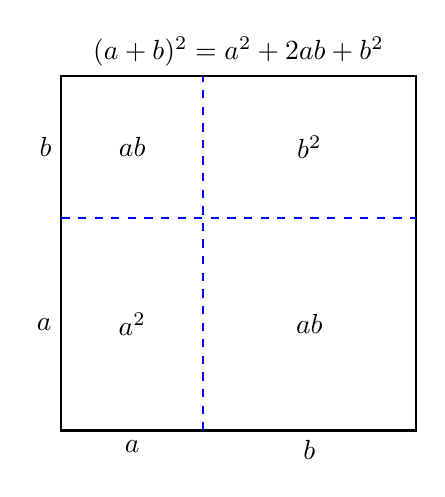
\begin{tikzpicture}[scale=0.9]
  % 大正方形 (a+b)^2
  \draw[thick] (0,0) rectangle (5,5);
  % 分割线
  \draw[thick, dashed, blue] (2,0) -- (2,5);
  \draw[thick, dashed, blue] (0,3) -- (5,3);
  % 标注边长
  \node[below] at (1,0) {$a$};
  \node[below] at (3.5,0) {$b$};
  \node[left] at (0,1.5) {$a$};
  \node[left] at (0,4) {$b$};
  % 标注四个区域
  \node at (1,1.5) {$a^2$};
  \node at (3.5,1.5) {$ab$};
  \node at (1,4) {$ab$};
  \node at (3.5,4) {$b^2$};
  % 总面积标注
  \node[above, font=\bfseries] at (2.5,5) {$(a+b)^2 = a^2 + 2ab + b^2$};
\end{tikzpicture}
\end{center}

\begin{warnbox}[易错提醒：完全平方公式的常见错误]
\begin{enumerate}[nosep]
  \item $(a + b)^2 \neq a^2 + b^2$（漏掉交叉项 $2ab$！这是最常见的错误！）
  \item $(a - b)^2 \neq a^2 - b^2$（同上，漏掉 $2ab$ 项）
  \item $(a + b)^2 \neq a^2 + ab + b^2$（交叉项应该是 $2ab$，不是 $ab$）
  \item $(a - b)^2 = a^2 - 2ab + b^2$，注意 $b^2$ 前面是正号（因为 $(-b)^2 = b^2$）
\end{enumerate}

\textbf{口诀：}首平方，尾平方，首尾二倍放中央；和的平方加中间，差的平方减中间。
\end{warnbox}

\begin{tipbox}[乘法公式的灵活运用]
\begin{itemize}[nosep]
  \item 平方差公式中的 $a$、$b$ 可以是单项式、多项式或数字。
  \item 例如：$(2x+3y)(2x-3y) = (2x)^2 - (3y)^2 = 4x^2 - 9y^2$
  \item 例如：$(x+y+z)(x-y-z) = [x+(y+z)][x-(y+z)] = x^2 - (y+z)^2$
  \item 完全平方公式的推广：$(a+b+c)^2 = a^2+b^2+c^2+2ab+2bc+2ac$
\end{itemize}
\end{tipbox}

% -------------------- 14.4 因式分解 --------------------
\subsection*{14.4\quad 因式分解}

\begin{knowledgebox}[因式分解的概念]
\textbf{定义：}把一个多项式化成几个整式的\textbf{积}的形式，叫做把这个多项式\textbf{因式分解}（或分解因式）。

\textbf{关键要点：}
\begin{enumerate}[nosep]
  \item 因式分解的对象是多项式（和的形式）。
  \item 因式分解的结果是整式的积的形式。
  \item 因式分解与整式乘法互为\textbf{逆运算}。
\end{enumerate}
$$\text{整式乘法：}(a+b)(a-b) \xrightarrow{\text{展开}} a^2 - b^2$$
$$\text{因式分解：}a^2 - b^2 \xrightarrow{\text{分解}} (a+b)(a-b)$$
\end{knowledgebox}

\begin{warnbox}[易错提醒：因式分解的注意事项]
\begin{enumerate}[nosep]
  \item 因式分解必须分解到\textbf{不能再分解}为止（分解彻底）。
  \item 结果必须是\textbf{积}的形式，不能是和差形式。
  \item $x^2 - 4 = (x+2)(x-2)$ 是因式分解（正确）。
  \item $x^2 - 4 = (x+2)(x-2) = x^2 - 4$ 不是因式分解（展开又回去了）。
  \item 注意公因式要提干净，首项系数为负时要提出负号。
\end{enumerate}
\end{warnbox}

\begin{knowledgebox}[提公因式法]
\textbf{方法：}如果多项式的各项有公因式，可以把这个公因式提到括号外面，将多项式写成公因式与另一个多项式的积。

$$\boxed{ma + mb + mc = m(a + b + c)}$$

\textbf{步骤：}
\begin{enumerate}[nosep]
  \item 找公因式：取各项系数的最大公因数，取各项相同字母的最低次幂。
  \item 提出公因式，将多项式写成公因式乘以剩余部分。
\end{enumerate}

\textbf{示例：}
$$6x^3y - 9x^2y^2 + 3x^2y = 3x^2y(2x - 3y + 1)$$
\end{knowledgebox}

\begin{knowledgebox}[公式法——平方差公式]
将平方差公式逆用：

$$\boxed{a^2 - b^2 = (a + b)(a - b)}$$

\textbf{适用条件：}两项，且每项都能写成完全平方的形式，中间是减号。

\textbf{示例：}
$$4x^2 - 25 = (2x)^2 - 5^2 = (2x+5)(2x-5)$$
\end{knowledgebox}

\begin{knowledgebox}[公式法——完全平方公式]
将完全平方公式逆用：

$$\boxed{a^2 + 2ab + b^2 = (a + b)^2}$$
$$\boxed{a^2 - 2ab + b^2 = (a - b)^2}$$

\textbf{适用条件：}三项，首尾两项是完全平方，中间项是首尾两项底数之积的$2$倍。

\textbf{示例：}
$$x^2 + 6x + 9 = x^2 + 2 \cdot x \cdot 3 + 3^2 = (x + 3)^2$$
$$4x^2 - 12xy + 9y^2 = (2x)^2 - 2 \cdot 2x \cdot 3y + (3y)^2 = (2x - 3y)^2$$
\end{knowledgebox}

\begin{tipbox}[因式分解的一般步骤]
\begin{enumerate}[nosep]
  \item \textbf{一看}：看各项有没有公因式，有则先提公因式。
  \item \textbf{二看}：提完公因式后，看能否用公式法（二项看平方差，三项看完全平方）。
  \item \textbf{三检查}：检查是否分解彻底，每个因式是否还能继续分解。
\end{enumerate}
\textbf{口诀：}一提（公因式）、二套（公式）、三查（是否彻底）。
\end{tipbox}

% -------------------- 十字相乘法（拓展） --------------------
\subsection*{14.5\quad 十字相乘法（拓展）}

\begin{knowledgebox}[十字相乘法]
对于二次三项式 $x^2 + (p+q)x + pq$，可以分解为：
$$\boxed{x^2 + (p+q)x + pq = (x + p)(x + q)}$$

\textbf{十字相乘图示：}
$$\begin{array}{ccc}
x & \xrightarrow{\quad} & p \\
\times & & \times \\
x & \xrightarrow{\quad} & q
\end{array}$$

交叉相乘：$x \cdot q + x \cdot p = (p+q)x$（等于一次项系数）。

\textbf{示例：}$x^2 + 5x + 6$

找两个数 $p$、$q$ 使得 $p + q = 5$ 且 $pq = 6$，得 $p = 2$、$q = 3$。

所以 $x^2 + 5x + 6 = (x+2)(x+3)$。
\end{knowledgebox}

\begin{tipbox}[十字相乘法的适用条件]
十字相乘法适用于形如 $x^2 + bx + c$ 的二次三项式（首项系数为$1$）。关键是找到两个数 $p$、$q$，使得：
\begin{itemize}[nosep]
  \item $p + q = b$（一次项系数）
  \item $p \cdot q = c$（常数项）
\end{itemize}
当 $c > 0$ 时，$p$、$q$ 同号（与 $b$ 同号）；当 $c < 0$ 时，$p$、$q$ 异号。
\end{tipbox}

% ==============================================================
% 第二部分：例题精讲
% ==============================================================
\section*{\textcolor{examorange}{二、例题精讲}}

\begin{examplebox}[【例题1】基础计算——幂的运算]
计算下列各式：

\textbf{(1)} $(-2a^2b)^3 \cdot 3ab^2$

\textbf{(2)} $(x^3)^2 \cdot x^5 \div x^4$
\end{examplebox}

\textbf{解：}

\textbf{(1)} $(-2a^2b)^3 \cdot 3ab^2$

$= (-2)^3 \cdot (a^2)^3 \cdot b^3 \cdot 3ab^2$

$= -8a^6b^3 \cdot 3ab^2$

$= (-8 \times 3) \cdot a^{6+1} \cdot b^{3+2}$

$= -24a^7b^5$

\medskip
\textbf{(2)} $(x^3)^2 \cdot x^5 \div x^4$

$= x^{3 \times 2} \cdot x^5 \div x^4$

$= x^6 \cdot x^5 \div x^4$

$= x^{6+5-4}$

$= x^7$

\begin{tipbox}[方法总结]
幂运算的关键是准确运用三条法则：同底数幂相乘（指数相加）、幂的乘方（指数相乘）、积的乘方（每个因式分别乘方）。混合运算时注意运算顺序，先乘方再乘除。
\end{tipbox}

\begin{examplebox}[【例题2】基础计算——整式乘法展开]
计算下列各式：

\textbf{(1)} $(3x - 2)(2x + 5)$

\textbf{(2)} $(x + 2y - 1)(x - 2y + 1)$
\end{examplebox}

\textbf{解：}

\textbf{(1)} $(3x - 2)(2x + 5)$

$= 3x \cdot 2x + 3x \cdot 5 + (-2) \cdot 2x + (-2) \cdot 5$

$= 6x^2 + 15x - 4x - 10$

$= 6x^2 + 11x - 10$

\medskip
\textbf{(2)} $(x + 2y - 1)(x - 2y + 1)$

观察结构：可以看作 $[x + (2y - 1)][x - (2y - 1)]$，符合平方差公式。

$= x^2 - (2y - 1)^2$

$= x^2 - (4y^2 - 4y + 1)$

$= x^2 - 4y^2 + 4y - 1$

\begin{tipbox}[方法总结]
多项式乘法展开时，先观察结构特征。如果能用乘法公式（平方差、完全平方），优先使用公式简化计算。第(2)题的关键是"分组"后识别出平方差公式的结构。
\end{tipbox}

\begin{examplebox}[【例题3】乘法公式的应用——化简求值]
先化简，再求值：$(2a + b)(2a - b) - (a - 2b)^2 + 5b(a - b)$，其中 $a = 2$，$b = -1$。
\end{examplebox}

\textbf{解：}

原式 $= [(2a)^2 - b^2] - [a^2 - 4ab + 4b^2] + 5ab - 5b^2$

$= 4a^2 - b^2 - a^2 + 4ab - 4b^2 + 5ab - 5b^2$

$= (4a^2 - a^2) + (4ab + 5ab) + (-b^2 - 4b^2 - 5b^2)$

$= 3a^2 + 9ab - 10b^2$

代入 $a = 2$，$b = -1$：

$= 3 \times 4 + 9 \times 2 \times (-1) - 10 \times 1$

$= 12 - 18 - 10$

$= -16$

\begin{tipbox}[方法总结]
化简求值问题的步骤：\textbf{先化简}（运用乘法公式展开、合并同类项），\textbf{后代入}求值。先化简可以减少计算量，降低出错概率。注意完全平方公式展开时不要漏掉交叉项。
\end{tipbox}

\begin{examplebox}[【例题4】证明题——乘法公式与恒等式]
证明：对任意正整数 $n$，$(n+1)^2 - n^2$ 的值总是一个奇数。
\end{examplebox}

\textbf{证明：}

$$(n+1)^2 - n^2$$

利用平方差公式：

$$= [(n+1) + n][(n+1) - n]$$

$$= (2n + 1) \times 1$$

$$= 2n + 1$$

因为 $n$ 是正整数，所以 $2n$ 是偶数，$2n + 1$ 是奇数。

所以对任意正整数 $n$，$(n+1)^2 - n^2 = 2n + 1$ 总是一个奇数。\qed

\begin{tipbox}[方法总结]
利用乘法公式可以简化代数式的证明。本题用平方差公式将平方差转化为一次式，比直接展开更简洁。这也说明了"连续两个正整数的平方差"等于这两个数之和（$2n+1$），这是一个常用结论。
\end{tipbox}

\begin{examplebox}[【例题5】易错辨析——因式分解中的常见错误]
判断下列因式分解是否正确，若有错误请改正：

\textbf{(1)} $x^2 - 9 = (x - 3)(x - 3)$

\textbf{(2)} $x^2 + 4x + 4 = (x + 4)^2$

\textbf{(3)} $2x^2 - 8 = 2(x^2 - 4)$（到此为止）

\textbf{(4)} $-x^2 + 6x - 9 = (x - 3)^2$
\end{examplebox}

\textbf{解：}

\textbf{(1)} 错误。

$x^2 - 9 = x^2 - 3^2$，用平方差公式得 $x^2 - 9 = (x+3)(x-3)$。

原解答写成了 $(x-3)^2 = x^2 - 6x + 9$，与原式不符。

\medskip
\textbf{(2)} 错误。

$(x+4)^2 = x^2 + 8x + 16 \neq x^2 + 4x + 4$。

正确做法：$x^2 + 4x + 4 = x^2 + 2 \cdot x \cdot 2 + 2^2 = (x+2)^2$。

\medskip
\textbf{(3)} 不彻底。

$2(x^2 - 4) = 2(x+2)(x-2)$，括号内的平方差还能继续分解。

\medskip
\textbf{(4)} 错误（符号处理错误）。

$-x^2 + 6x - 9 = -(x^2 - 6x + 9) = -(x - 3)^2$。

原解答没有提出负号，导致结果符号错误。注意 $(x-3)^2 = x^2 - 6x + 9$，与原式 $-x^2 + 6x - 9$ 恰好相反。

\begin{warnbox}[易错提醒总结]
\begin{enumerate}[nosep]
  \item 平方差公式 $a^2 - b^2 = (a+b)(a-b)$，两因式一个加一个减，不是两个都减。
  \item 完全平方公式要看清中间项：$(x+2)^2 = x^2 + 4x + 4$，不是 $(x+4)^2$。
  \item 因式分解要分解彻底，不能"半途而废"。
  \item 首项系数为负时，先提出负号再分解。
\end{enumerate}
\end{warnbox}

\begin{examplebox}[【例题6】综合提高——巧用乘法公式计算]
不用计算器，计算下列各式：

\textbf{(1)} $102 \times 98$

\textbf{(2)} $51^2 - 49^2$
\end{examplebox}

\textbf{解：}

\textbf{(1)} $102 \times 98$

$= (100 + 2)(100 - 2)$

$= 100^2 - 2^2$ \quad（平方差公式）

$= 10000 - 4$

$= 9996$

\medskip
\textbf{(2)} $51^2 - 49^2$

$= (51 + 49)(51 - 49)$ \quad（平方差公式）

$= 100 \times 2$

$= 200$

\begin{tipbox}[方法总结]
乘法公式在简便计算中非常实用。看到两个数相乘且它们的和或差为整十整百，就可以尝试平方差公式。看到两个大数的平方差，用平方差公式比直接计算更高效。
\end{tipbox}

\begin{examplebox}[【例题7】交叉综合——因式分解与等腰三角形（第13章）]
已知 $a$、$b$、$c$ 是 $\triangle ABC$ 的三边长，且满足 $a^2 - 2ab + b^2 = 0$。试判断 $\triangle ABC$ 的形状。
\end{examplebox}

\textbf{解：}

$a^2 - 2ab + b^2 = 0$

左边用完全平方公式因式分解：

$(a - b)^2 = 0$

所以 $a - b = 0$，即 $a = b$。

因为 $a = b$，$\triangle ABC$ 是以 $a$、$b$ 为腰的\textbf{等腰三角形}。

\begin{tipbox}[方法总结]
本题将因式分解与第13章的等腰三角形判定联系起来。核心思路：通过因式分解将条件转化为边的关系（$a = b$），再根据等腰三角形的判定（两边相等的三角形是等腰三角形）得出结论。因式分解是代数与几何之间的桥梁。
\end{tipbox}

% ==============================================================
% 第三部分：应用题
% ==============================================================
\section*{\textcolor{apppurple}{三、应用题}}

\begin{appbox}[【应用1】面积问题——花园扩建]
一个正方形花坛的边长为 $a$ 米，现在要在花坛的四边各向外扩展 $b$ 米，形成一个新的大正方形。求扩展后花坛面积比原来增加了多少平方米。
\end{appbox}

\textbf{解：}

原花坛面积 $= a^2$（平方米）。

扩展后花坛边长 $= a + 2b$（每边各向外扩展 $b$ 米，两边加 $2b$）。

扩展后花坛面积 $= (a + 2b)^2 = a^2 + 4ab + 4b^2$（平方米）。

增加的面积 $= (a + 2b)^2 - a^2 = a^2 + 4ab + 4b^2 - a^2 = 4ab + 4b^2 = 4b(a + b)$（平方米）。

\textbf{答：}扩展后花坛面积增加了 $4b(a + b)$ 平方米。

\begin{tipbox}[方法总结]
面积变化问题通过用代数式表示变化前后的面积，再利用乘法公式展开、化简求差。这类问题很好地体现了整式乘法在实际问题中的应用。
\end{tipbox}

\begin{appbox}[【应用2】数字规律——连续奇数之和]
用因式分解说明：对于任意正整数 $n$，$1 + 3 + 5 + \cdots + (2n-1) = n^2$。
\end{appbox}

\textbf{解：}

左边是首项为 $1$、末项为 $2n-1$、项数为 $n$ 的等差数列之和。

用等差数列求和公式：
$$S = \frac{(\text{首项} + \text{末项}) \times \text{项数}}{2} = \frac{[1 + (2n - 1)] \times n}{2} = \frac{2n \times n}{2} = n^2$$

所以 $1 + 3 + 5 + \cdots + (2n-1) = n^2$。

\textbf{验证：}
\begin{itemize}[nosep]
  \item $n=1$：$1 = 1^2$，成立。
  \item $n=2$：$1+3 = 4 = 2^2$，成立。
  \item $n=3$：$1+3+5 = 9 = 3^2$，成立。
  \item $n=5$：$1+3+5+7+9 = 25 = 5^2$，成立。
\end{itemize}

\textbf{几何解释：}从 $1$ 开始的 $n$ 个连续奇数之和恰好等于 $n \times n$ 的正方形中所含的点数。每一个新的奇数对应正方形"外围新增的一圈"。

\begin{tipbox}[方法总结]
代数中的恒等式常有优美的几何解释。前 $n$ 个奇数之和等于 $n^2$，这个结论可以通过等差数列求和（代数方法）或正方形点阵（几何方法）两种方式理解。
\end{tipbox}

\begin{appbox}[【应用3】材料节省——管道截面设计]
一根圆形钢管的外径为 $D$，内径为 $d$（壁厚为 $\dfrac{D - d}{2}$）。钢管横截面的面积（环形面积）为 $\dfrac{\pi(D^2 - d^2)}{4}$。用因式分解说明：当外径不变、内径增大时，截面积如何变化，并计算 $D = 10$ cm，$d$ 从 $6$ cm 增大到 $8$ cm 时截面积减少了多少（结果保留 $\pi$）。
\end{appbox}

\textbf{解：}

截面积公式：$S = \dfrac{\pi(D^2 - d^2)}{4}$

用平方差公式因式分解：

$$S = \frac{\pi(D + d)(D - d)}{4}$$

当 $D$ 不变、$d$ 增大时：
\begin{itemize}[nosep]
  \item $(D + d)$ 增大（因为 $d$ 增大）；
  \item $(D - d)$ 减小（因为 $d$ 增大）。
\end{itemize}

但从物理意义来看，内径增大意味着壁变薄，截面积（金属面积）减少。

当 $D = 10$ cm，$d_1 = 6$ cm 时：
$$S_1 = \frac{\pi(10^2 - 6^2)}{4} = \frac{\pi(100 - 36)}{4} = \frac{64\pi}{4} = 16\pi \text{ (cm}^2\text{)}$$

当 $D = 10$ cm，$d_2 = 8$ cm 时：
$$S_2 = \frac{\pi(10^2 - 8^2)}{4} = \frac{\pi(100 - 64)}{4} = \frac{36\pi}{4} = 9\pi \text{ (cm}^2\text{)}$$

截面积减少了 $S_1 - S_2 = 16\pi - 9\pi = 7\pi \text{ (cm}^2\text{)}$。

\textbf{答：}截面积减少了 $7\pi$ cm$^2$（约 $21.99$ cm$^2$）。

\begin{tipbox}[方法总结]
工程计算中，平方差公式可以将 $D^2 - d^2$ 分解为 $(D+d)(D-d)$，这有助于分析变量变化对结果的影响趋势。因式分解不仅是代数技巧，更是分析问题的有力工具。
\end{tipbox}

% ==============================================================
% 第四部分：课堂练习
% ==============================================================
\section*{\textcolor{tipgreen}{四、课堂练习}}

\begin{enumerate}
  \item 计算：$(-3a^2b)^2 \cdot 2ab^3$

  \item 计算（用乘法公式）：$(3x + 2y)(3x - 2y)$

  \item 因式分解：$4x^2 - 12xy + 9y^2$

  \item 因式分解：$2x^3 - 8x$

  \item 先化简再求值：$(a + 2b)(a - 2b) - (a - b)^2$，其中 $a = 3$，$b = -2$。
\end{enumerate}

\vspace{10pt}

\begin{knowledgebox}[参考答案]

\textbf{第1题：}

$(-3a^2b)^2 \cdot 2ab^3$

$= 9a^4b^2 \cdot 2ab^3$

$= 18a^5b^5$

\medskip
\textbf{第2题：}

$(3x + 2y)(3x - 2y) = (3x)^2 - (2y)^2 = 9x^2 - 4y^2$

\medskip
\textbf{第3题：}

$4x^2 - 12xy + 9y^2$

$= (2x)^2 - 2 \cdot 2x \cdot 3y + (3y)^2$

$= (2x - 3y)^2$

\medskip
\textbf{第4题：}

$2x^3 - 8x$

$= 2x(x^2 - 4)$

$= 2x(x + 2)(x - 2)$

注意：要先提公因式 $2x$，再对括号内的平方差继续分解，共需两步。

\medskip
\textbf{第5题：}

原式 $= a^2 - 4b^2 - (a^2 - 2ab + b^2)$

$= a^2 - 4b^2 - a^2 + 2ab - b^2$

$= 2ab - 5b^2$

代入 $a = 3$，$b = -2$：

$= 2 \times 3 \times (-2) - 5 \times 4$

$= -12 - 20$

$= -32$

\end{knowledgebox}

\vfill
\begin{center}
\small\textcolor{gray}{本讲义仅供教学参考，例题可根据学生水平调整难度。}
\end{center}

\end{document}
